\section{Schwerebeschleunigung}

Die Gravitationsbeschleunigung aufgrund der Anziehung zweier Massen ist
\begin{equation}
 \vec{b}_a(\vec{r})=G\int_V \frac{\rho(\vec{r}')}{|\vec{r}'-\vec{r}|^3}(\vec{r}'-\vec{r})\text{d}V'
\end{equation}
mit der Gravitationskonstanten
\begin{equation}
 G=\eb{6,673\cdot 10^{-11}}{m^3}{kg\,s^2} \fullstop
\end{equation}

Außerdem wirken noch scheinbare Schwerewirkungen wie zum Beispiel die Zentrifugalbeschleunigung $\vec{z}(\vec{r})$, die durch die Erdrotation hervorgerufen wird.

Wird eine Messung der Schwere durchgeführt, wird immer die vektorielle Summe dieser beiden Beschleunigungen
\begin{equation}
 \vec{g}_a(\vec{r})=\vec{b}_a(\vec{r})+\vec{z}(\vec{r})
\end{equation}
gemessen.

Die SI-Einheit der Schwerebeschleunigung ist $\left[g\right]=\eb{1}{m}{s^2}$, wobei in der Geophysik meist die Einheit $\e{1}{Gal}$ verwendet wird. Die Umrechnung erfolgt durch
\begin{equation}
 \eb{1}{m}{s^2}=\e{100}{Gal} \fullstop
\end{equation}

\section{Reduktionen}
\label{sec:Reduktionen}

Meist möchte man durch die gemessenen Schwereunterschiede auf einen unbekannten Dichteunterschied im Untergrund schließen. Dazu müssen jedoch die bekannten Schwereunterschiede aus den Messwerten eliminiert werden. Es wird von Reduktion der Schwerewerte gesprochen.

Die Freiluftreduktion (oder auch Niveaureduktion) $\q{\delta}{g\,Niv}$ berücksichtigt, dass die Schwere mit zunehmender Höhe $H$ abnimmt. Es gilt dabei
\begin{equation}
 \q{\delta}{g\,Niv}=\eb{-0,3086\cdot H}{mGal}{m} \fullstop
 \label{eq:Freiluft}
\end{equation}
Den gleichen Effekt muss man bei der Instrumentenhöhe beachten, was zu $\q{\delta}{g\,Instrumentenhoehe}$ führt. Die Instrumentenhöhe wird jedoch direkt bei der Messung aus den Messwerten eliminiert, weil dies eine von der Geometrie der Messung unabhängige Auswertung ermöglicht.

Bei der Gezeitenreduktion $\q{\delta}{g\,Gez}$ wird die Gravitationswirkung anderer Planeten berücksichtigt, die sich mit der Zeit verändert.

Die Driftreduktion $\q{\delta}{g\,Drift}$ muss durchgeführt werden, weil sich die Eigenschaften der Bauteile des Gravimeters mit der Zeit ändern können. Um diese Änderung erfassen zu können, wird an allen Messpunkten mindestens zweimal gemessen. Dadurch kann eine Funktion interpoliert bestimmt werde, die die Drift im Laufe der Zeit darstellt. Diese Korrektur muss auf jeden Fall nach der Gezeitenkorrektur durchgeführt werden, damit alle anderen zeitlichen Veränderungen schon aus der Messung eliminiert sind.

Die Geländereduktion $\q{\delta}{g\,Gel}$ berücksichtigt die Verringerung des Schwerewerts durch zum Beispiel Berge und Täler in der Nähe des Messorts. Nach der Korrektur ist der Messwert also vergrößert.

Die Bouguerreduktion berücksichtigt den Effekt, dass eine Gesteinsschicht zwischen Referenzfläche und Messpunkt den gemessenen Wert der Schwere vergrößert. Es wird angenommen, dass diese Gesteinsschicht aus homogenem Material der Dichte $\rho$ besteht. Dies führt zur Gleichung
\begin{equation}
 \q{\delta}{g\,Bouguer}=2\pi\rho GH=\eb{0,0419\cdot H\cdot\rho\cdot 10^{-8}}{m^3}{s^2kg}
\end{equation}
für diese Reduktion.

Die Breitenreduktion beinhaltet die räumlichen Schwereunterschiede aufgrund der breitenabhängigen Zentrifugalbeschleunigung, die durch die Erdrotation hervorgerufen wird. Der Schwerewert vergrößert sich hierbei mit zunehmender Breite. Die Normalschwereformel
\begin{equation}
 \q{\delta}{g\,Breite}=\eb{8,2\cdot L\cdot 10^{-9}}{1}{s^2}
\end{equation}
liefert mit dem Abstand $L$ zur geographischen Breite des Referenzpunkts den Korrekturwert.

% regionale Reduktion das gleiche???
Die geologische Reduktion $\q{\delta}{g\, geol}$ beachtet den überregionalen Trend nach der Karte der Bougueranomalien von Baden-Württemberg. Sie kann aus dem Rechts- und Hochwert mit Formel
\begin{equation}
 \q{\delta}{g\, geol}=\left( 0,000953\cdot \Delta\q{L}{Hoch} - 0,00055 \cdot \Delta\q{L}{Rechts} \right) \eb{}{mGal}{m}
\end{equation}
bestimmt werden. Der Rechtswert $\Delta\q{L}{Rechts}$ ist der Fortschritt in Ostrichtung bezüglich eines gewählten Referenzpunkts.
Der Hochwert $\Delta\q{L}{Hoch}$ ist der Fortschritt in Nordrichtung bezüglich des gleichen Referenzpunkts. Beide Größen haben die Einheit Meter.

Von einer Bougueranomalie $\q{g}{Bouguer}$ wird gesprochen, wenn all diese Reduktionen auf den Messwert $\q{g}{mess}$ angewendet wurden. Es gilt also
% regio???
\begin{align}
 \q{g}{Bouguer}=\q{g}{mess}-\q{\delta}{g\,Instrumentenhoehe}-\q{\delta}{g\,Gez}-\q{\delta}{g\,Drift}-\q{\delta}{g\,Gel} \\ \notag
 -\q{\delta}{g\,Niv}-\q{\delta}{g\,Breite}-\q{\delta}{g\,Bouguer}
 -\q{\delta}{regio}
\end{align}

\section{Messinstrumente}

\subsection{Gravimeter}

Im Versuch werden LaCoste-Romberg G-Gravimeter benutzt. Der Aufbau eines solchen Gravimeters ist in Abbildung \ref{fig:grav} zu sehen. Das grundlegende Prinzip ist, dass sich eine an einer Feder hängende Masse im Schwerefeld der Erde befindet und die unterschiedliche Auslenkung der Masse an unterschiedlichen Orten oder zu unterschiedlichen Zeiten gemessen wird. Diese Gravimeter können also Differenzen von Schwerebeschleunigungen messen, aber keine Absolutwerte.

\begin{figure}
    \centering
   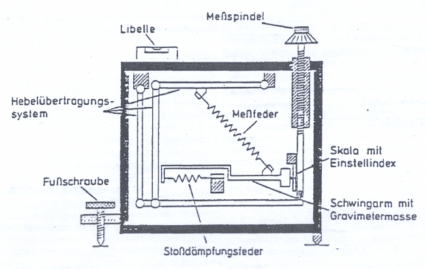
\includegraphics[width=0.7\textwidth]{fig/gravimeter}
 \caption[Aufbau eines LaCoste-Romberg G-Gravimeters]{Aufbau eines LaCoste-Romberg G-Gravimeters \cite{skript}}
 \label{fig:grav}
\end{figure}

In der Ruhelage befindet sich der Schwingarm mit Gravimetermasse in der Horizontalen. Ändert sich dann die Schwere, wird die Masse anders ausgelenkt und die Masse kann durch Drehen an der Messspindel wieder in die Ausgangslage gebracht werden. Die Anzahl der notwendigen Spindelumdrehungen $U$ ist proportional zur Schwereänderung $\Delta g$
\begin{equation}
 \Delta g= U\cdot p
\end{equation}
mit einem geräteabhängigen Proportionalitätsfaktor $p$.
% Andere Buchstaben???

Ein Gravimeter hat eine Messempfindlichkeit von $\e{0,01}{mGal}$, weswegen das Gerät sehr gut gegen physikalische Nebeneffekte geschützt werden muss. Es ist zum Beispiel mit einem Thermostat auf ein Hundertstel Grad temperaturstabilisiert, druckdicht gebaut und magnetisch abgeschirmt. Trotzdem ist eine sehr sorgfältige Messung wichtig, um brauchbare Ergebnisse zu erhalten. 

\subsection{Tachymeter}

Obwohl die Höhenbestimmung beim Nivellement genauer ist, wird in diesem Versuch die Höhe mit einer Totalstation bestimmt. Es handelt sich dabei um eine Kombination aus einem Tachymeter und einem elektronischen Entfernungsmesser. Mit einem Fernrohr wird der Punkt anvisiert, dessen Höhe gegenüber der Totalstation gemessen werden soll. Dadurch ist der Winkel $\alpha$ gegenüber der Horizontalen bekannt (siehe Abbildung ???). Außerdem wird am zu vermessenden Punkt ein Reflektor angebracht. Dadurch wird ein vom elektronischen Entfernungsmesser ausgehender Laserstrahl zurück geschickt und mit der Laufzeit $t$ und der Lichtgeschwindigkeit $c$ kann mit der Formel
\begin{equation}
 s=c\cdot \frac{t}{2}
\end{equation}
die Entfernung $s$ berechnet werden. Dies geschieht direkt im Gerät. Aus der Länge $s$ kann direkt die Höhendifferenz
\begin{equation}
 \Delta h=\sin(\alpha)\cdot s
\end{equation}
bestimmt werden. 
% Abbildung Prinzip Tachymeter einfügen

\subsection{Global Navigation Satellite System (GNSS)}

Mit GNSS werden Höhenmessungen durchgeführt und die während der Messungen markierten Pflöcke eingemessen. Das Prinzip beruht darauf, dass 

% differentielles GPS soll hier beschrieben werden!!!